\documentclass{article}

\usepackage[version=3]{mhchem}
\usepackage{amsmath}
\usepackage{authblk}

\newcommand{\metabalize}{\texttt{metabalize }}
\newcommand{\readmzfile}{\texttt{read\_mz\_file}}
\newcommand{\toydeisotope}{\texttt{toy\_deisotope}}
\newcommand{\testtoydeisotope}{\texttt{toy\_deisotope}}


\title{Initial directions for the \texttt{metabalize} package}
\author{Drew}

\usepackage{Sweave}
\begin{document}
\maketitle
\Sconcordance{concordance:initial_directions.tex:initial_directions.Rnw:%
1 15 1 1 0 3 1 1 5 15 1 1 2 1 0 1 2 6 0 1 2 2 1 1 2 1 0 1 1 7 0 1 2 3 1 %
1 2 1 0 1 2 7 0 1 1 9 0 1 2 6 1 1 2 1 0 1 3 24 0 2 2 5 0 1 2 14 1}



\section{Functions}

The \metabalize package currently exists in embryonic form. There are three functions:

\begin{itemize}
  \item \readmzfile, which reads a .csv or .xlsx file generated by MAVEN, and returns the data frame containing the results. Currently this is a little silly, but the idea is to develop it in the future to create objects which are slightly less trivial.
  Note to self: converting m/z values from double to integer doesn't seem to help much - object size is reduced by half, and there's a performace gain of maybe 50\% at lower numbers of peaks, but at higher number of peaks the performance gain goes away. 
  \item \toydeisotope, a `toy' version of the planned deisotoping function. Currently it identifies peaks that differ in median m/z by a specified amount (\texttt{mass\_diff}), plus or minus a tolerance (\texttt{tolerance}), meaning that it can only identify one isotopomer. (The default is a difference of a single \ce{^{13}C}, +/- 2e-5).
  \item \testtoydeisotope This tests the \textit{performance} of \toydeisotope (not its accuracy). The algorithm behind \toydeisotope scales as $O(n^2)$, i.e., the time it takes is proportional to the square of the number of peaks analyzed. I need to make the algorithm more efficient; standard testing will me to track those efforts.
\end{itemize}

\section{Workflow}

First, load a data set using \readmzfile. \texttt{"maven-output.csv"} contains a 193-peak data set of known compounds produced by MAVEN:

\begin{Schunk}
\begin{Sinput}
> mz_df <- read_mz_file("../data/maven-output.csv")
> nrow(mz_df)
\end{Sinput}
\begin{Soutput}
[1] 193
\end{Soutput}
\end{Schunk}

Second, identify isotopomers. Currently \toydeisotope can only look for one isotopomer at a time (currently the defaults are set to a difference of a single \ce{^{13}C} with tolerance of $2 \times 10^{-5}$ m/z). It will be straightforward to add multiple isotopomers; the tricky thing is finding a good search algorithm.

\begin{Schunk}
\begin{Sinput}
> is_short <- toy_deisotope(mz_df)
> is_short
\end{Sinput}
\begin{Soutput}
[1] mz1 mz2
<0 rows> (or 0-length row.names)
\end{Soutput}
\end{Schunk}
OK, this data set doesn't seem to have any isotopomers, assuming I've set the tolerance correctly. Have they been removed already?

Let's check a dataset of unknown peaks to see whether we can find some isotopomers. We don't want to check the whole dataset for istopomers - this creates a 12 Gb memory object, as currently written - but we can check the first thousand elements for isotopes.

\begin{Schunk}
\begin{Sinput}
> unknowns <- read_mz_file("../data/maven-output-unknowns.csv")
> system.time({
+   unknown_isotopes <- toy_deisotope(unknowns[1:1000, ])})
\end{Sinput}
\begin{Soutput}
   user  system elapsed 
  1.063   0.090   1.162 
\end{Soutput}
\begin{Sinput}
> print(unknown_isotopes)
\end{Sinput}
\begin{Soutput}
            mz1      mz2
765058 87.00810 88.01147
852077 89.02377 90.02712
852078 89.02377 90.02712
\end{Soutput}
\end{Schunk}

So this says that the peak at 87.00810 has an isotopomer at 88.01147, and the peak at 89.02377 has two isotopomers at 90.02712 (which have different retention times.)

\section{Performance}

Let's look in a little more detail at the performance of \toydeisotope. We'll take successively larger data sets (all subsampled from \texttt{unknowns}). As mentioned above, the time should scale about as $n^2$.

\begin{Schunk}
\begin{Sinput}
> subset_lengths=seq(from=500, to=4000, by=250)
> system.time({
+   performance <- test_toy_deisotope(unknowns, subset_lengths=subset_lengths)
+ })
\end{Sinput}
\begin{Soutput}
[1] 0.069 0.041 0.111
[1] 0.347 0.054 0.405
[1] 0.766 0.089 0.862
[1] 0.990 0.133 1.137
[1] 1.220 0.196 1.426
[1] 1.64 0.28 1.95
[1] 1.818 0.332 2.185
[1] 2.390 0.477 2.902
[1] 2.872 0.616 3.533
[1] 3.435 0.765 4.274
[1] 3.932 0.969 5.024
[1] 4.667 1.565 7.188
[1]  5.190  2.428 17.284
[1]  5.753  2.137 16.751
[1]  7.191  4.101 31.607
   user  system elapsed 
 43.425  16.025  99.692 
\end{Soutput}
\end{Schunk}

\begin{Schunk}
\begin{Sinput}
> plot(performance[ , "subset_lengths"], performance[, "elapsed"], xlab="number of elements", ylab="elapsed time, s")
\end{Sinput}
\end{Schunk}
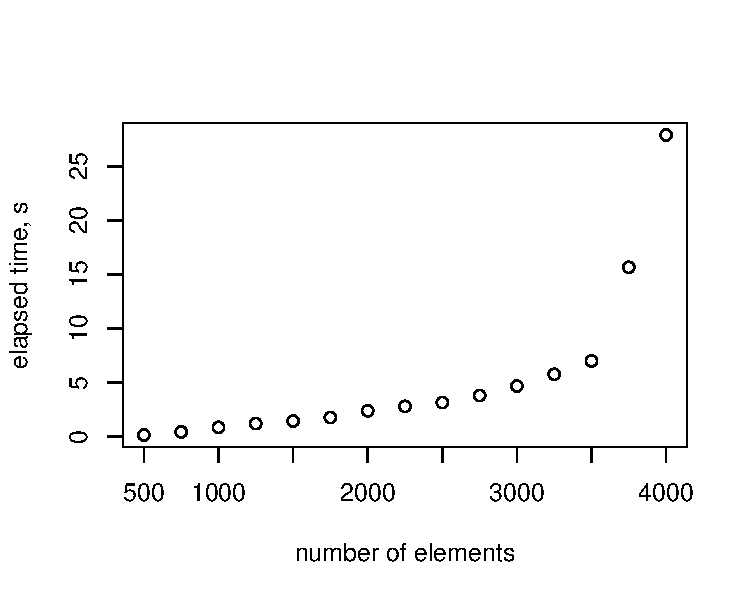
\includegraphics{initial_directions-performanceFig}

Two observations:
\begin{enumerate}
  \item The times get big, quick. Above, say, 5000, this method will require a bigger computer.
  \item The required time appears to increase somewhat faster than $n^2$
\end{enumerate}

So, clearly this approach won't work for large data sets, although it works fine for smaller ones. I can see two ways to address this:

\begin{itemize}
  \item Rewrite some of the deisotoping code in C++ using the \texttt{Rcpp} package. This might save a little time, but probably won't save too much.
  \item Change the algorithm so that, rather than comparing every m/z value against every other m/z value, it eliminates impossible comparisons ahead of time. One possibility would be to split the data set into overlapping bins based on elution time, so that peaks with very different elution times would not be compared to each other. 
\end{itemize}

\end{document}
